
\documentclass[hide notes,intlimits]{beamer}


\mode<presentation>
{
  \usetheme[headline,footline]{UAFshade}
  \setbeamercovered{transparent}
}

% load packages
\usepackage[english]{babel}
\usepackage[latin1]{inputenc}
\usepackage[T1]{fontenc}
\usepackage{multimedia}
\usepackage{lmodern}
\usepackage[amssymb]{SIunits}
%\usepackage{hyperref}
\bibliographystyle{andy}


% NOTE:
% Instead of pgf, you can also use the familiar \includegraphics commad





% title page
\title[Glacier Dynamics] % (optional, use only with long paper titles)
{Mechanics and Thermodynamics of Glaciers}
\subtitle{Glaciers 617}


\author[Aschwanden] % (optional, use only with lots of authors)
{Andy Aschwanden}
% - Give the names in the same order as the appear in the paper.
% - Use the \inst{?} command only if the authors have different
%   affiliation.

\institute[ARSC] % (optional, but mostly needed)
{
  %
  Arctic Region Supercomputing Center\\
  University of Alaska Fairbanks, USA
}
% - Use the \inst command only if there are several affiliations.
% - Keep it simple, no one is interested in your street address.




\subject{Glaciers}

% define what is shown at the beginning of each section
\AtBeginSection[]
{
 \begin{frame}<beamer>
   \frametitle{Outline}
   \tableofcontents[currentsection,subsectionstyle=hide/show/hide]
 \end{frame}
}

% define what is shown at the beginning of each subsection
\AtBeginSubsection[]
{
 \begin{frame}<beamer>
  \frametitle{Outline}
   \tableofcontents[currentsection,currentsubsection]
 \end{frame}
}

\begin{document}

% insert titlepage
\begin{frame}
  \titlepage
\end{frame}

% insert TOC
\begin{frame}
 \frametitle{Outline}
 \tableofcontents[subsectionstyle=hide]
  %You might wish to add the option [pausesections]
\end{frame}

\section{Introduction}


\begin{frame}
  \frametitle{Recall from Vector Calculus}
  \begin{block}{Divergence Theorem}
    \begin{equation}
      \oint_{\partial \omega} \boldsymbol{\phi} \,\text{d}a = 
      \int_{\omega} \nabla \cdot \boldsymbol{\phi} \, \text{d} v
    \end{equation}
  \end{block}
  \begin{block}{Reynolds Tranport Theorem}
    \begin{equation}
     \frac{\text{d}}{\text{d} t}\int_{\omega} \boldsymbol{\phi}\, \text{d} v =
     \int_{\omega} \frac{\partial \boldsymbol{\phi}}{\partial{t}} \, \text{d} v +
      \oint_{\partial \omega} \boldsymbol{\phi} \mathbf{v}\cdot\mathbf{n}\,\text{d}a 
    \end{equation}
  \end{block}
\end{frame}


\begin{frame}
  \frametitle{My Favorite Reference}
  Greve,~R., and H.~Blatter: Dynamics of Ice Sheets and Glaciers. Springer, 2009.
  \begin{itemize}
    \item notation follows closely
  \end{itemize}
\end{frame}


\begin{frame}
  \frametitle{Why}
  The flow of glaciers and ice sheets is an interesting, non-trival problem in fluid dynamics
\end{frame}

{
\setbeamertemplate{headline}[default]
\begin{frame}
  \frametitle{Why}
  The flow of glaciers and ice sheets is an interesting, non-trival problem in fluid dynamics
\end{frame}
}   

\begin{frame}
  \frametitle{Concepts}
 \begin{itemize}
    \item material objectivity
  \end{itemize}
\end{frame}

\begin{frame}
  \frametitle{Questions}
  \centering{
    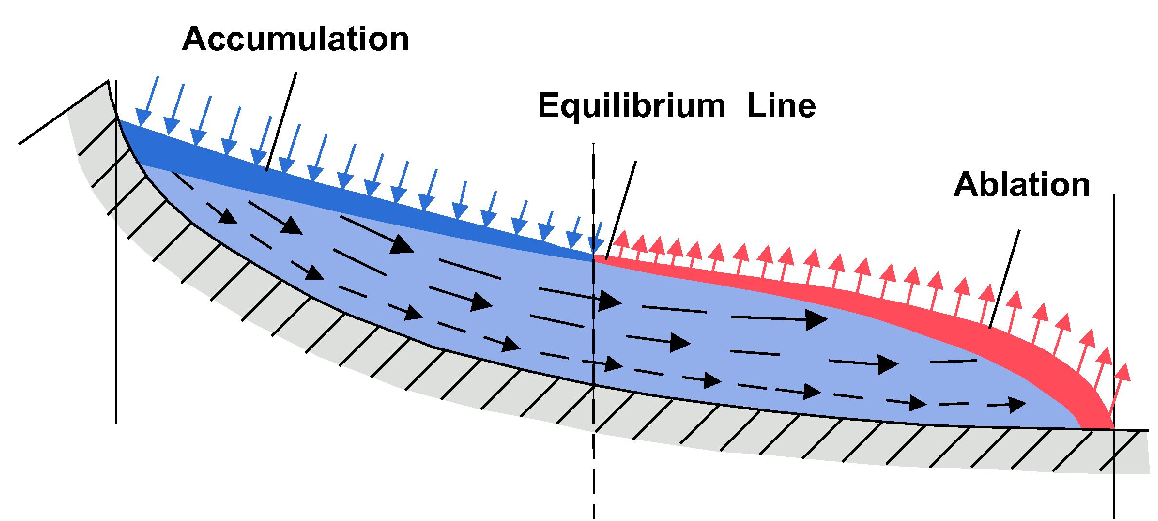
\includegraphics[width=.5\textwidth]{figures/flow_acc_abl}
  }
 \begin{itemize}
    \item What determines the glacier shape and extend
    \item How do ablation, accumulation, ice temperature, and the bedrock topography influence the flow of a glacier
    \item How does the flow speed vary with depth, along a flowline, or orthogonal to a flowline
  \end{itemize}
\end{frame}

\begin{frame}
  \frametitle{Questions}
  \centering{
    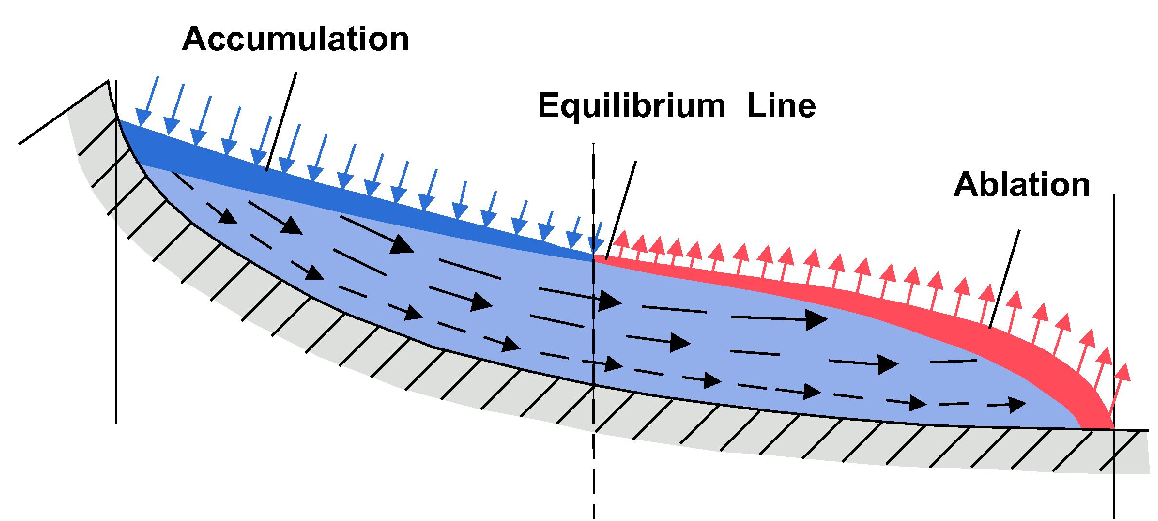
\includegraphics[width=.5\textwidth]{figures/flow_acc_abl}
  }
 \begin{block}{The two major problems}
   \begin{enumerate}
   \item Given the boundary conditions,
     \begin{itemize}
     \item basal topography
     \item accumulation-ablation function
     \item temperature at the upper ice surface
     \item geothermal heat flux at the base,
   \end{itemize}
   which glacier (geometry) is in equilibrium for given bc's.
  \item How does the glacier respond to changes in the bc's?
\end{enumerate}
  \end{block}
\end{frame}

\begin{frame}
  \frametitle{Answer}
  \centering{
    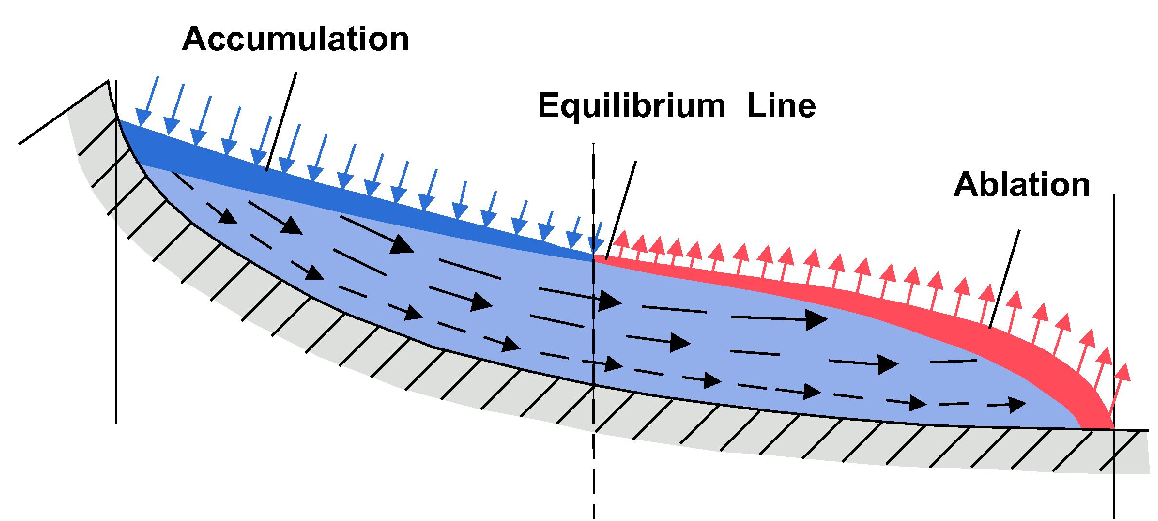
\includegraphics[width=.5\textwidth]{figures/flow_acc_abl}
  }

 \begin{block}{Solution: Continuums Mechanics}
   Solve balance equations for
 \begin{itemize}
    \item mass
    \item linear and angular momentum
    \item energy
    \item (forget about entropy)
    \end{itemize}
  \end{block}
\end{frame}

\section{Balance Equations}

\begin{frame}
  \frametitle{General Balance Equations}
  \begin{equation*}
   \frac{\partial g}{\partial t} = - \nabla \cdot \left(\boldsymbol{\phi} + g\mathbf{v}\right) + p + s
 \end{equation*}
 \begin{columns}
   \column[C]{0.1cm}
   $g$ \\
   $\boldsymbol{\phi}$ \\
   $p$ \\
   $s$ \\
   \column[C]{6cm}
   physical quantity \\
   flux of $g$ through the boundary \\
   production of $g$ \\
   supply of $g$
 \end{columns}
\end{frame}


\begin{frame}
  \frametitle{Balance Equations}
  \large{
  \begin{equation*}
  \begin{array}{lcclc}
    \text{mass} \quad &  \frac{\text{d} \rho}{\text{d} t} & = & -\rho\nabla \cdot \mathbf{v} \quad & (1)\\[.25em]
    \text{momentum} \quad & \frac{\text{d} \mathbf{v}}{\text{d} t} & = & -\nabla \cdot \mathbf{T} - \mathbf{f} \quad & (3) \\[.25em]
    \text{internal energy} \quad & \frac{\text{d} u}{\text{d} t} & = & - \nabla \cdot \mathbf{q} + \text{tr} \left(\mathbf{T}\cdot\mathbf{D}\right) \quad & (1)
  \end{array}
  \end{equation*}
  }
\centering{
 \begin{columns}
   \column[T]{4cm} \centering{
   left-hand side \\
   $\rho$ (1)\\
   $\mathbf{v}$ (3)\\
   $u$ (1)
   }
   \column[T]{4cm} \centering{
   right-hand side \\
   $\mathbf{T}$ (6)\\
   $\mathbf{q}$ (3)
  }
 \end{columns}
  }
  \begin{itemize}
   \item so we have 5 equations for 14 unknown fields
   \item the system is highly under-determined
   \item[$\Rightarrow$] \alert{closure relations} required
 \end{itemize}
\end{frame}

\begin{frame}
  \frametitle{Closure Relations}
  \begin{itemize}
    \item \alert{balance equations} are universally valid
    \item \alert{closure relations} describe the specific behavior of a material
    \item \alert{closure relations} are often called \alert{constitutive equations}
  \end{itemize}
\end{frame}


\begin{frame}
  \frametitle{Balance Equations for Glaciers}
  \large{
  \begin{equation*}
  \begin{array}{lcclc}
    \text{mass} &  \nabla \cdot \mathbf{v} & = & 0 \quad & (3)\\
    \text{momentum} & \nabla \cdot \mathbf{T} & = & - \rho \mathbf{g} \quad & (3)\\
    \text{internal energy} & \frac{\text{d} u}{\text{d} t} & = & - \nabla \cdot \mathbf{q} + \text{tr}\left(\mathbf{T}\cdot\mathbf{D}\right) \quad & (1)
  \end{array}
  \end{equation*}
  }
\centering{
 \begin{columns}
   \column[T]{4cm} \centering{
   left-hand side \\
   $\mathbf{v}$ (3)\\
   $\mathbf{T}$ (6)\\
   $u$ (1)
   }
   \column[T]{4cm} \centering{
   right-hand side \\
  $\mathbf{q}$ (3)
  }
 \end{columns}
  }
  \begin{itemize}
   \item so we have 7 equations for 13 unknown fields
   \item the system is highly under-determined
   \item[$\Rightarrow$] \alert{closure relations} required
 \end{itemize}
\end{frame}

\section{Constitutive Equations}

\begin{frame}
  \frametitle{Constitutive Equations for Glaciers}
  \begin{itemize}
    \item for the heat flux $\mathbf{q}$
    \item for the viscosity $\eta$
  \end{itemize}
\end{frame}


\begin{frame}
  \frametitle{Constitutive Equations for Glaciers}
  \begin{itemize}
    \item ask a material scientist or rheologist
    \item and let him/her do some fancy experiments
 \end{itemize}
\end{frame}

\begin{frame}
  \frametitle{Constitutive Equations for Glaciers}
  From experiments, you will learn that ice behaves like a
  \begin{itemize}
    \item viscous
    \item non-Newtionian
    \item heat-conduction
 \end{itemize}
fluid. So what does this mean?
\end{frame}

\begin{frame}
  \frametitle{Constitutive Equations for Glaciers}
  \begin{block}{Viscous material}
 \begin{itemize}
    \item deformation rate $\propto$ stress
\end{itemize}
 \end{block}
  \begin{block}{Non-Newtonian fluid}
 \begin{itemize}
    \item non-linear relationship between deformation rate and stress
\end{itemize}
 \end{block}
\end{frame}

\section{Glaciers and Ice Sheets}

\begin{frame}
  \frametitle{Large-Scale Dynamics}
  Some typical values
  \begin{equation*}
  \begin{array}{rccl}
    \text{horizontal extend} &  [L] & = & \unit{1000}\kilo\meter\\
    \text{vertical extend} & [H] & = & \unit{1}\kilo\meter \\
    \text{horizontal velocity} & [U] & = & \unit{100}\meter\power{a}{-1}\\
    \text{vertical velocity} & [W] & = & \unit{0.1}\meter\power{a}{-1}\\
    \text{pressure} & [U] & = & \rho g[H] = \unit{10}\mega\pascal\\
    \text{time-scale} & [T] & = &[L]/[U] = 10^{4}\usk\power{a}{1}\\
  \end{array}
  \end{equation*}
  The aspect ratio $\epsilon$ is defined as
  \begin{equation*}
    \epsilon = \frac{[H]}{[L]} = \frac{[U]}{[W]} = 10^{-3} \text{ for an ice sheet}
  \end{equation*}
\end{frame}

\end{document}


